\section{Section: Prelude}

\section{Section Intro}

\begin{frame}[c]{Der Plan}
  \small

  \begin{enumerate}
    \item \textbf{Was ist Kryptografie}
    \item \textbf{Endzeitstimmung (Quantenattacken)}
    \item \textbf{Migration zu Post-Quanten-Kryptografie}
    \item \textbf{Werbesendung (Die Migration im Eigenen Betrieb)}
  \end{enumerate}

	\vfill
	\qrcode[height=2.5cm]{https://github.com/rosenpass/slides/blob/main/2025-05-15-cast/slides.pdf}~Folien \hfill Full~Paper~\qrcode[height=2.5cm]{https://doi.org/10.1007/s13272-025-00806-5}

  \vfill
\end{frame}



\begin{frame}{Karolin Varner}
  \begin{columns}[fullwidth,c]
	\hspace*{.25\LeftSlideIndent}%
    \begin{column}{\dimexpr.7\linewidth-.25\LeftSlideIndent}
      \begin{itemize}
        \item Initiatorin \& Leiterin des Rosenpass e.V.
        \item Software-Entwicklerin \& Kryptografin
        \item 12 Jahre in der Industrie bei Startups und Konzernen
        \item Seit 2024 am Max-Planck-Institut für Sicherheit und Privatsphäre
        \item Arbeit an Rosenpass \& weiteren kryptografischen Projekten wie zum Beispiel der X-Wing~Chiffre
      \end{itemize}
    \end{column}%
    \begin{column}{.3\linewidth}
      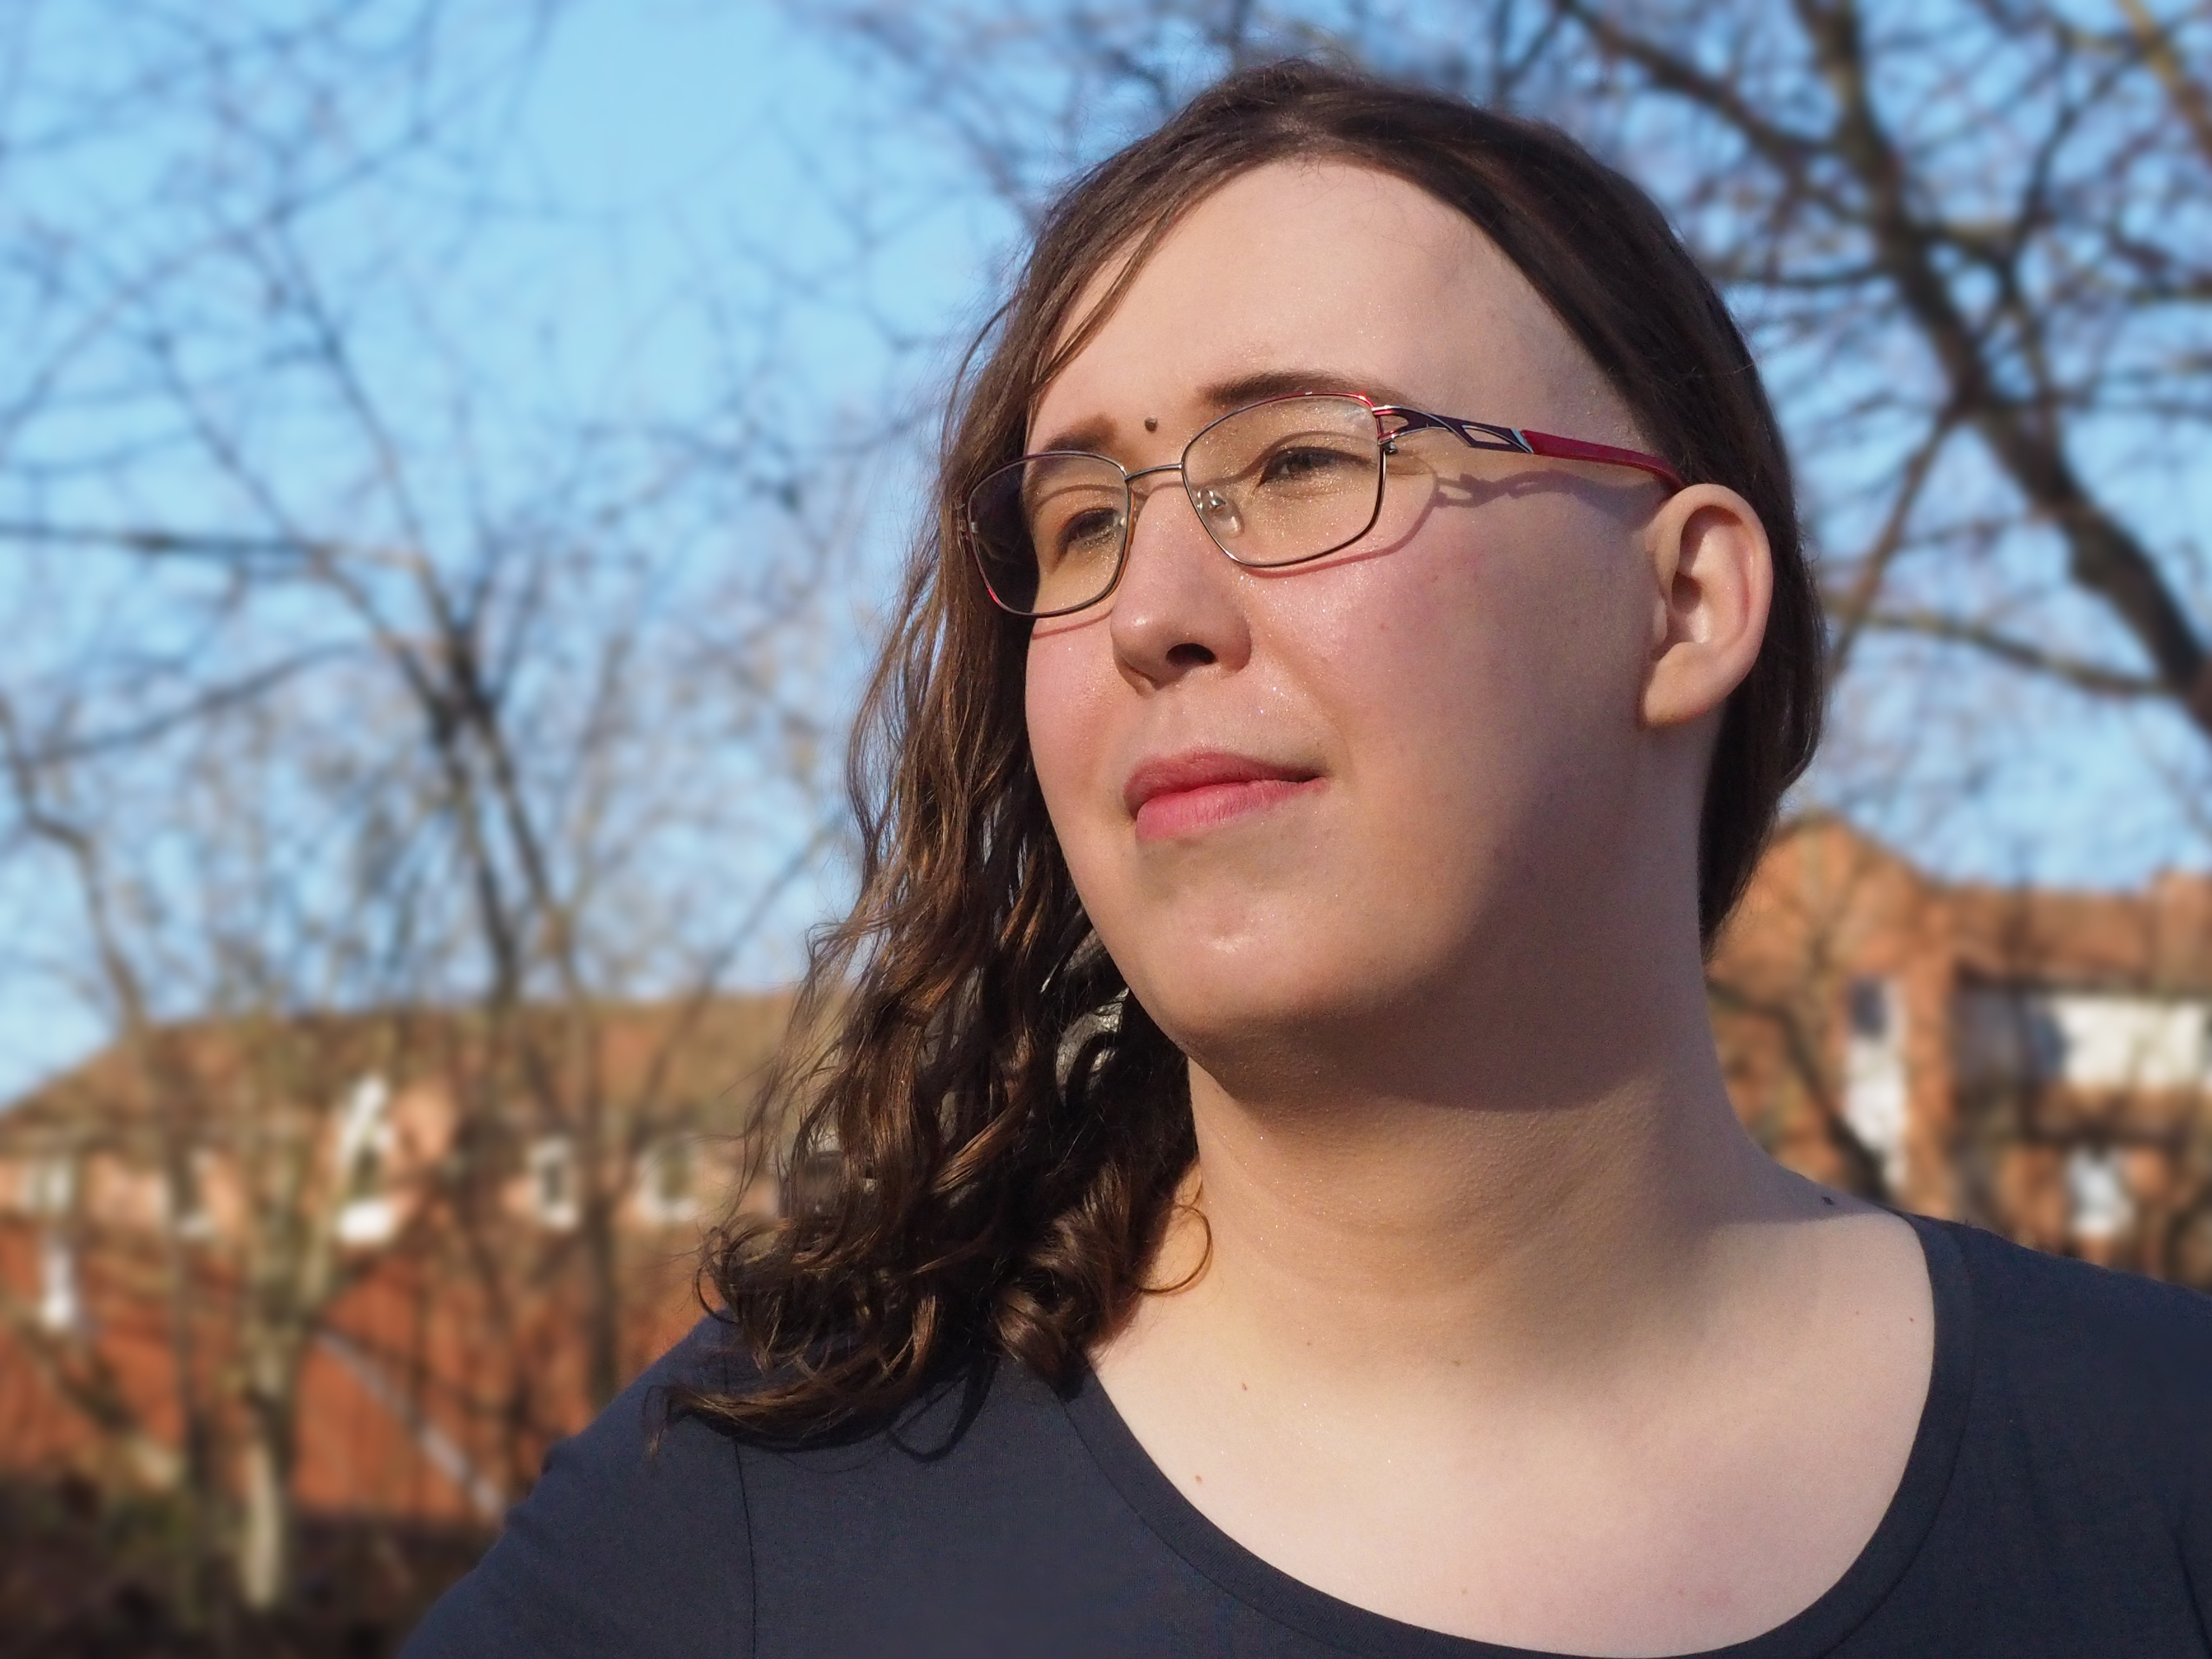
\includegraphics[width=.92\linewidth,trim=200 0 100 0,clip]{graphics/karolin-varner.jpg}
    \end{column}
  \end{columns}
\end{frame}

\begin{frame}{Rosenpass e.V.}
  \begin{columns}[fullwidth,c]
  	\hspace*{.25\LeftSlideIndent}
    \begin{column}{.5\linewidth}
      \begin{itemize}
        \item 2023 gegründet zur Betreuung des gleichnamigen Projekts
        \vfill
        \item Absicherung von WireGuard gegen Attacken durch Quantencomputer mittels protocol-level Hybridisierung
        \item Institution für Translationsforschung in der Kryptografie
        \vfill
        \item Schnittstelle zwischen Forschung, Industrie und Gesellschaft
      \end{itemize}
      \bigskip
      \textbf{\url{rosenpass.eu}}
    \end{column}%
    \begin{column}{.5\linewidth}
%      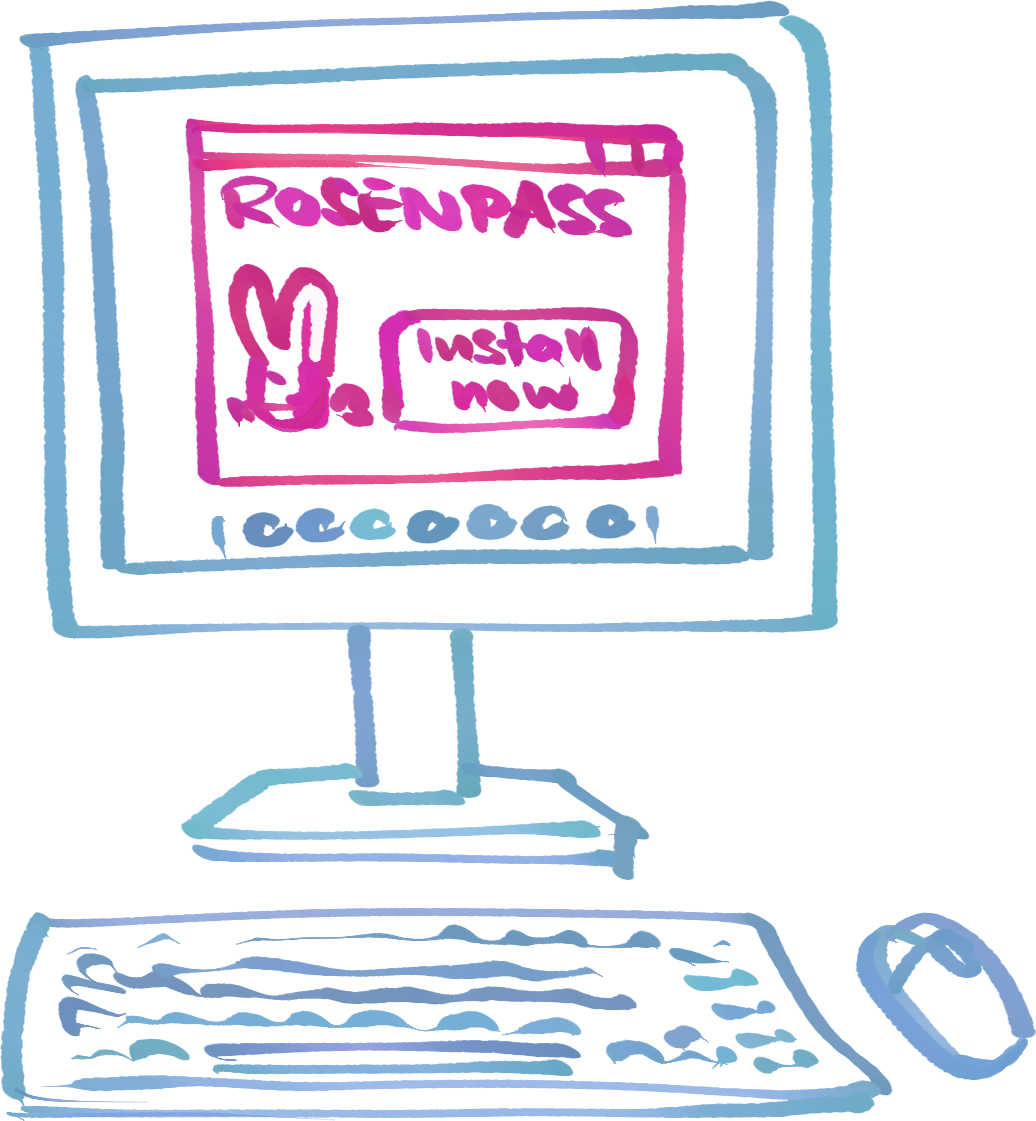
\includegraphics[ width=.92\linewidth]{graphics/Illu-install.png}
		\makebox[\linewidth][c]{\includegraphics[width=1.3\linewidth,page=18]{hpke-slide-designs}\hskip1.5em}
    \end{column}%
  \end{columns}
\end{frame}
